\documentclass[a4paper, 12pt]{article}
\usepackage{graphicx}
\usepackage[margin=1in]{geometry}
\usepackage{titlesec}
\usepackage{indentfirst}
\usepackage{setspace}
\usepackage{amsmath}
\usepackage{amssymb}
\usepackage[outputdir = ../]{minted}
\usepackage[svgnames]{xcolor}
\usepackage[hidelinks]{hyperref}
\usepackage{tabularray}
\usepackage{graphbox}
\usepackage{float}
\usepackage{comment}
\usepackage{longtable,booktabs,array}
\usepackage{calc}
\usepackage{subfig}
\usepackage[
    backend=biber,
    style=authoryear,
  ]{biblatex}
\addbibresource{bib.bib}

\titleformat{\section}[block]{\large\bfseries}{\thesection}{0.5cm}{}
\titleformat{\subsection}[block]{\normalfont\bfseries}{\thesubsection}{0.5cm}{}
\titlespacing{\subsection}{8pt}{8pt}{8pt}

\newcommand\mefvm{%
    \textit{m}\kern-.1em%
    \raise0.5ex\hbox{\textit{e}}\kern-.1em%
    \textit{f}\kern-.2em%
    \raise-0.5ex\hbox{\textit{v}}\kern-.05em%
    \textit{m}
}
\renewcommand{\labelitemi}{-}
\renewcommand{\labelitemii}{-}

\begin{document}
\doublespacing
\begin{titlepage}
    \begin{center}
        
\includegraphics[width=0.8\textwidth]{university1.jpg}\\
        
        \textbf{ME485: Computational Fluid Dynamics \\ Using Finite Volume Method}

        \vspace{0.5cm}
        Homework 2
            
        \vspace{1.5cm}

        \textbf{Uğur Ozan Baygeldi}\\
        \textbf{Ali Kaya}\\ 
        \textbf{Onur Kakilli}\\~\\
        Group 15
        
    \end{center}
\end{titlepage}

\section{Introduction}

This report is on the second homework of the course ME485, Computational Fluid Dynamics Using Finite Volume Method. The homework requests some implementations of diffusion methods to \mefvm\!. \nocite{gi}

\section{Roadmap}

This report follows a route mentioned in the previous homework of Group 15, which is initially looking at the \verb|system.py| file and implementing the methods requested as the methods appear on the code. (\cite{hw1}) The purpose of this homework is to complete the missing parts of the code such that the following are implemented successfully:
\begin{itemize}
    \item Implement \verb|_make_compute_fpts| and \verb|_make_grad| to \verb|ParabolicElements| class at \verb|elements.py|
    \item Implement \verb|make_grad_at_face| and \verb|_make_flux| to \verb|ParabolicIntInters| and \\ \verb|ParabolicBCInters| classes at \verb|inters.py|
    \item Implement \verb|_make_compute_norm| to \verb|elements.py|
 \end{itemize}\par
Although there are arguably fewer requests from the previous Homework, a tough and challenging path remains to be solved.

\section{Implementation of \texttt{\_make\_grad} and \texttt{\_make\_compute\_fpts} at\\\texttt{elements.py}}

\subsection{Implementation of \texttt{\_make\_compute\_fpts}}
\verb|_make_compute_fpts| is implemented the same as the previous homework. The code simply assigns cell center values to every face of an element. This is generally the first step in the CFD methods.\\\par

The implemented code:
\begin{minted}[frame=lines,framesep=2mm,baselinestretch=1.2,bgcolor=Cornsilk,fontsize=\footnotesize,linenos]{python}
    def _make_compute_fpts(self):
        nvars, nface = self.nvars, self.nface
        def _compute_fpts(i_begin, i_end, upts, fpts):
            # Code taken directly from HW1
            for idx in range(i_begin, i_end):
                for j in range(nvars):
                    for i in range(nface):
                        fpts[i, j, idx] = upts[j, idx]
        return self.be.make_loop(self.neles, _compute_fpts)
\end{minted}

\subsection{Implementation of \texttt{\_make\_grad}}
Similarly, the code is exactly the same with the previous homework. Unlike the previous homework, in the method uses Least Squares to determine the gradient which from the outcomes of the last homework was determined to work better in general.\\\par

The code for the operator is, once again, the same used in the previous homework. As implementing the operator is not requested, the code for the operator will not be shared to prevent bulk.\\\par

The code:
\begin{minted}[frame=lines,framesep=2mm,baselinestretch=1.2,bgcolor=Cornsilk,fontsize=\footnotesize,linenos]{python}
    def _make_grad(self):
        nface, ndims, nvars = self.nface, self.ndims, self.nvars
        # Gradient operator 
        op = self._prelsq
        def _cal_grad(i_begin, i_end, fpts, grad):
            # Code taken directly from HW1
            for idx in range(i_begin, i_end):
                for d in range(ndims):
                    for j in range(nvars):  # = 1
                        sum = 0
                        for i in range(nface):
                            sum += fpts[i, j, idx] * op[d, i, idx]

                        grad[d, j, idx] = sum
        return self.be.make_loop(self.neles, _cal_grad)   
\end{minted}

\section{Implementation of \texttt{\_make\_flux} and \texttt{\_make\_grad\_at\_face} at \texttt{inters.py}}


\subsection{Mathematical Implementation of \texttt{\_make\_flux}}
In orthogonal structure, if \(e\) represents the unit vector along the
direction defined by the line connecting nodes \(e\ and\ ef\):
\begin{equation}
    e = \frac{\mathbf{r}_{ef} - \mathbf{r}_{e}}{\left\| \mathbf{r}_{ef} - \mathbf{r}_{e} \right\|} = \frac{\mathbf{d}_{e - ef}}{d_{e - ef}}
\end{equation}
\begin{equation}
    (\nabla\phi.e)_{f} = \left( \frac{\partial\phi}{\partial e} \right)_{f} = \frac{\phi_{ef} - \phi_{e}}{\left\| \mathbf{r}_{ef} - \mathbf{r}_{e} \right\|} = \frac{\phi_{ef} - \phi_{e}}{d_{e - ef}}
\end{equation} \par
To linearize the flux equation in non-orthogonal structures the surface
vector \(\mathbf{S_{f}}\) can be written as summation of two vectors \(\mathbf{E_{f}}\) and \(\mathbf{T_{f}}\). \par
\begin{equation}
    \mathbf{S}_{f} = \mathbf{E}_{f} + \mathbf{T}_{f}
\end{equation} \par
The above equation can be rewritten as follows:
\begin{equation}
    (\nabla\phi)_{f}\cdot S_{f} = (\nabla\phi)_{f}\cdot\mathbf{E}_{f} + \ (\nabla\phi)_{f} \cdot \mathbf{T}_{f}
\end{equation}
\begin{equation}(\nabla\phi)_{f}\cdot\mathbf{E}_{f} = E_{f}\frac{\phi_{ef} - \phi_{e}}{\left\| \mathbf{r}_{ef} - \mathbf{r}_{e} \right\|}\ 
\end{equation}
\begin{equation}
    (\nabla\phi)_{f}\cdot S_{f} = E_{f}\frac{\phi_{ef} - \phi_{e}}{\left\| r_{ef} - r_{e} \right\|} + \ (\nabla\phi)_{f}\cdot\mathbf{T}_{f}
\end{equation}\par
To calculate \(\mathbf{E_{f}}\) one can use the following approaches. \\\par

\begin{longtable*}[]{@{}
  >{\raggedright\arraybackslash}p{(\columnwidth - 2\tabcolsep) * \real{0.5000}}
  >{\raggedright\arraybackslash}p{(\columnwidth - 2\tabcolsep) * \real{0.5000}}@{}}
\toprule()
\begin{minipage}[b]{\linewidth}\raggedright
Approach
\end{minipage} & \begin{minipage}[b]{\linewidth}\raggedright
Implementation of \(\mathbf{E_{f}}\)
\end{minipage} \\
\midrule()
\endhead
(a) Minimum Correction & \(\mathbf{E_{f}} = \left( \mathbf{e} \cdot S_{f} \right) \mathbf{e} \) \\
(b) Orthogonal Correction & \(\mathbf{E_{f}} = S_{f}\mathbf{e}\) \\
(c) Over-Relaxed Correction & \(\mathbf{E_{f}} = \dfrac{S_{f}}{\mathbf{e} \cdot \mathbf{n_{f}}}\mathbf{e}\) \\
\bottomrule()
\end{longtable*}

\begin{figure*}
 \centering
 \label{fig:images}
 \subfloat[Minimum]{%
      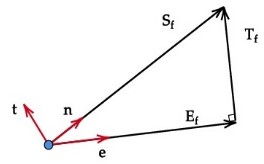
\includegraphics[width=0.25\textwidth]{image1}}
      \label{fig:image-a}
 \qquad
 \subfloat[Orthogonal]{%
      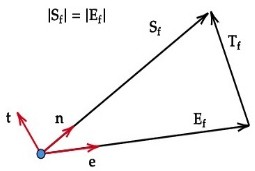
\includegraphics[width=0.25\textwidth]{image2}}
      \label{fig:image-b}
 \qquad
 \subfloat[Over-Relaxed]{%
      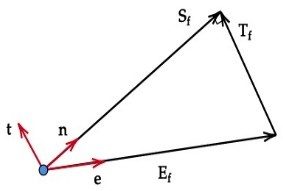
\includegraphics[width=0.25\textwidth]{image3}}
      \label{fig:image-c}
\end{figure*} 
\newpage
Taken from lecture notes part-8 (\cite{lect}). With a small correction to the over-relaxed method taken from an online source (\cite{cor}).

\subsection{Code Implementation of \texttt{\_make\_flux}}
To implement \verb|_make_flux| with appropriate corrections the following code is utilized for \verb|ParabolicIntInters| class:

\begin{minted}[frame=lines,framesep=2mm,baselinestretch=1.2,bgcolor=Cornsilk,fontsize=\footnotesize,linenos]{python}
    def _make_flux(self, nele):
        ndims, nfvars = self.ndims, self.nfvars
        lt, le, lf = self._lidx
        rt, re, rf = self._ridx
        nf, sf = self._vec_snorm, self._mag_snorm
        # Inverse distance between the elements
        inv_ef    = self._rcp_dx
        # Unit vector connecting cell centers 
        ef = self._dx_adj * inv_ef
        # Correction method to be used
        correction = self._correction
        # Compiler arguments
        array = self.be.local_array()
        # Get compiled function of viscosity and viscous flux
        compute_mu = self.ele0.mu_container()
        
        def comm_flux(i_begin, i_end, muf, gradf, *uf):
            # Parse element views (fpts, grad)
            du = uf[:nele]
            for idx in range(i_begin, i_end):
                mu = compute_mu()
                fn = 0.0
                Sf = nf[:,idx] * sf[idx]
                lti, lei, lfi = lt[idx], le[idx], lf[idx]
                rti, rei, rfi = rt[idx], re[idx], rf[idx]
                
                if correction == 'minimum':
                    # Ef = (Sf dot e) * e
                    Ef = dot(ef[:,idx], Sf, ndims)
                elif correction == 'orthagonal':
                    Ef = sf[idx]
                elif correction == 'over-relaxed':
                    Ef = (dot(Sf, Sf, ndims)/dot(Sf, ef[:, idx], ndims))
                    # https://www.cfd-online.com/Wiki/Diffusion_term 
                else:
                    print("Wrong Correction")
                    
                Tf = Sf - Ef * ef[:, idx]
                for k in range(nfvars):
                    fn = -1 * mu * (Ef * (du[lti][lfi, k, lei] * inv_ef[idx])
                                    + dot(gradf[:, k, idx], Tf, ndims))

                    uf[lti][lfi, k, lei] =  fn
                    uf[rti][rfi, k, rei] = -fn
                    
        return self.be.make_loop(self.nfpts, comm_flux)
\end{minted} 
\par
Notice how there is a selector that changes $E_f$ according to the correction method used. To save some calculations and implement the flux easier the magnitude is calculated, to obtain $\mathbf{E_f}$, in $\mathbf{T_f}$ for example, the magnitude is multiplied by the $\mathbf{e}$ vector. \\\par

The method is similar for the boundary elements however with a small addition of calling the \verb|bc| function. \\\par

The code for \verb|_make_flux| at \verb|ParabolicBCInters| class:

\begin{minted}[frame=lines,framesep=2mm,baselinestretch=1.2,bgcolor=Cornsilk,fontsize=\footnotesize,linenos]{python}
    def _make_flux(self, nele):
        ndims, nfvars = self.ndims, self.nfvars
        lt, le, lf = self._lidx
        nf, sf = self._vec_snorm, self._mag_snorm
        # Mangitude and direction of the connecting vector
        inv_ef = self._rcp_dx
        ef = self._dx_adj * inv_ef
        # Correction method to be used
        correction = self._correction
        # Compiler arguments
        array = self.be.local_array()
        # Get compiled function of viscosity and viscous flux
        compute_mu = self.ele0.mu_container()
        # Get bc function 
        bc = self.bc

        def comm_flux(i_begin, i_end, muf, gradf, *uf):
            # Parse element views (fpts, grad)
            du    = uf[:nele]
            # Same as int but with no right element
            for idx in range(i_begin, i_end):
                Sf = nf[:, idx] * sf[idx]
                muf = compute_mu()
                fn = 0.0
                lti, lei, lfi = lt[idx], le[idx], lf[idx]
                
                if correction == 'minimum':
                    # Ef = (Sf dot e) * e
                    Ef = dot(Sf, ef[:, idx], ndims)
                elif correction == 'orthagonal':
                    Ef = sf[idx] # * ef[:, idx]
                elif correction == 'over-relaxed':
                    Ef = (dot(Sf, Sf, ndims)/dot(Sf, ef[:, idx], ndims))
                    # https://www.cfd-online.com/Wiki/Diffusion_term 
                else:
                    print("Wrong Correction")
                    
                Tf = Sf - Ef * ef[:, idx]
                for k in range(nfvars):
                    ur = array(nfvars)
                    nfi = nf[:, idx]
                    bc(du[lti][lfi, k, lei],ur,nfi)
                    fn = -1 * muf * (Ef * (du[lti][lfi, k, lei] * inv_ef[idx]) 
                                     + dot(gradf[:, k, idx], Tf, ndims))

                    uf[lti][lfi, k, lei] = fn
                
        return self.be.make_loop(self.nfpts, comm_flux)
\end{minted} 
\par
Unlike the \verb|ParabolicIntInters| class, this implementation additionally runs the \verb|bc| function to obtain the values of the imaginary right element. However, whether this step is necessary or not is up to debate.
\subsection{Implementation of \texttt{\_make\_grad\_at\_face}}
As explained in the homework document the gradient at face is calculated using weights. 
\begin{equation}
    (\nabla q)_{face} = \omega_l(\nabla q)_{left\:element} +\omega_r(\nabla q)_{right\:element} 
\end{equation}

Which is implemented easily as the weights are already calculated previously by the \verb|compute_weight| function. \\\par

The code is as follows for the \verb|ParabolicIntInters| class:

\begin{minted}[frame=lines,framesep=2mm,baselinestretch=1.2,bgcolor=Cornsilk,fontsize=\footnotesize,linenos]{python}
    def _make_grad_at_face(self, nele):
        nvars, ndims = self.nvars, self.ndims
        lt, le, lf = self._lidx
        rt, re, rf = self._ridx    
        # Inverse distance between the cell center
        weight    = self._weight
        # Stack-allocated array
        array = self.be.local_array()

        def grad_at(i_begin, i_end, gradf, *uf):
            # Parse element views (fpts, grad)
            du    = uf[:nele]
            gradu = uf[nele:]
            for idx in range(i_begin, i_end):
                lti, lei, lfi = lt[idx], le[idx], lf[idx]
                rti, rei, rfi = rt[idx], re[idx], rf[idx]
                for j in range(nvars):
                    for i in range(ndims):
                        # weight of right = 1 - weight of left
                        gradf[i, j, idx] = weight[idx]*gradu[lti][i, j, lei] 
                        + (1 - weight[idx])*gradu[rti][i, j, rei]

        return self.be.make_loop(self.nfpts, grad_at)   
\end{minted}

Similarly for the \verb|ParabolicBCInters| class as no boundary gradient data is needed, the right elements gradient at cell center is set as the face gradient.

\begin{minted}[frame=lines,framesep=2mm,baselinestretch=1.2,bgcolor=Cornsilk,fontsize=\footnotesize,linenos]{python}
    def _make_grad_at_face(self, nele):
        nvars, ndims = self.nvars, self.ndims
        lt, le, lf = self._lidx

        # Mangitude and direction of the connecting vector
        inv_tf = self._rcp_dx                            # This code was left here
        tf = self._dx_adj * inv_tf                       # probably unintentionally.
        avec = self._vec_snorm/np.einsum('ij,ij->j', tf, self._vec_snorm)

        # Stack-allocated array
        array = self.be.local_array()

        def grad_at(i_begin, i_end, gradf, *uf):
            du    = uf[:nele]
            gradu = uf[nele:]
            # Same as int but with no right element
            for idx in range(i_begin, i_end):
                lti, lei, lfi = lt[idx], le[idx], lf[idx]
                for j in range(nvars):
                    for i in range(ndims):
                        gradf[i, j, idx] = gradu[lti][i, j, lei]

        return self.be.make_loop(self.nfpts, grad_at) 
\end{minted}

\section{Implementation of \texttt{\_make\_compute\_norm}}

\subsection{Mathematical Implementation of \texttt{\_make\_compute\_norm}}
The heat flux caused by a temperature difference $T_2 - T_1$ on a disk can be calculated analytically. The heat flux between the inner radius ($r_1$) and the outer radius ($r_2$) is determined using the following expressions.\\\par

The radial distance $r_i$ of any element on the disk can be calculated as shown below, where \(x_0\) and \(x_1\) represent the x and y coordinates of the elements.
\begin{equation}
    r_i = \sqrt{x_0^2 + x_1^2}
\end{equation} \par
The radial heat flux $q$ is calculated using the formula:
\begin{equation}
q = -\dfrac{\mu_f (T_2 - T_1)}{r_i \ln\left(\dfrac{r_2}{r_1}\right)}
\end{equation} \par

The divergence of the temperature gradient (heat flux) enables the analysis of heat generation, dissipation or accumulation within a system. This information is essential for characterizing and optimizing heat transfer in complex geometries or materials with variable thermal conductivity. \\\par The divergence of the heat flux, can be  expressed analytically as:

\begin{equation}
\nabla \cdot(\mu_f \:\nabla \cdot \vec{q}) = -\mu_f (T_2 - T_1) \left( \dfrac{(x_0 - x_1)(x_0 + x_1)}{r_i \ln\left(\dfrac{r_2}{r_1}\right)} + \dfrac{x_1^2 - x_0^2}{r_i \ln\left(\dfrac{r_2}{r_1}\right)} \right)
\end{equation} \par
With the exact solution known, the error could be calculated for radial meshes. \\\par

To measure the accuracy of the solution, $L_2$ norm of error will be used which is calculated as such:
\begin{equation}
\text{Error} = (\nabla \cdot(\mu_f \:\nabla \cdot \vec{q}))_\text{numerical} - (\nabla \cdot(\mu_f \:\nabla \cdot \vec{q}))_\text{analytical}
\end{equation} \par
The total error for all elements and variables is transformed into a norm as follows:
\begin{equation}
\text{$L_2$ norm} = \sqrt{\sum_{i=0}^{n} \text{Error}_i^2 \cdot V_{i}}
\end{equation} \par
The methodology explained above is applied to the square mesh (Kershaw Mesh) with an equation for exact temperature taken from the beloved ME311 Heat Transfer course book. (\cite{inc})\\\par

It is found that when calculated the divergence of flux is equal to 0 for square meshes after tedious implementation of the code. Or in other terms:
\begin{equation}
    (\nabla \cdot(\mu_f \:\nabla \cdot \vec{q}))_\text{analytical} = 0
\end{equation}
\subsection{Code Implementation of \texttt{\_make\_compute\_norm}}
The code that implements the $L_2$ norm of error calculation for meshes with internal radius $0.1\sqrt{2}$ and outer radius $1\sqrt{2}$ with inner and outer boundary conditions of 0 and 1 is shown on the next page.
\begin{minted}[frame=lines,framesep=2mm,baselinestretch=1.2,bgcolor=Cornsilk,fontsize=\footnotesize,linenos]{python}
    def _make_compute_norm(self):
        # Code taken directly from HW1
        nvars, neles, ndims = self.nvars, self.neles, self.ndims
        vol = self._vol
        xcs = self.xc
        #T2g = self.cfg.get('soln-bcs-outer', 'q')
        #T1g = self.cfg.get('soln-bcs-inner', 'q') # there was an attempt made
        muf = 1

        def run(upts):
            err = np.zeros((nvars, neles))
            T2, T1 = 1, 0
            L, W = 1, 1
            r = [0.1 * (2 ** 0.5), 1 * (2 ** 0.5)]
            for idx in range(neles):
                x = np.zeros(ndims)
                for i in range(nvars):
                    for j in range(ndims):
                        x[j] = xcs[idx][j]

                    # Regular Disk
                    r_i = (x[0] ** 2 + x[1] ** 2) ** 0.5
                    flux = - (muf*(T2-T1))/(r_i*np.log(r[1]/r[0])) 
                    # incropera c.5 eqn is div of flux
                    eqn = -muf*(T2-T1)*(((x[0]-x[1])*(x[0]+x[1]))
                                        /(np.log(r[1]/r[0])*r_i)
                    +((x[1]**2-x[0]**2))/(np.log(r[1]/r[0])*r_i))
                    err[i,idx] = ((upts[i, idx] - eqn)**2)*vol[idx]

                    # Kershaw
                    '''sumx, sumy = 0, 0
                    for f in range(1,31): # set up arbitrary infinite sum
                        top = np.sinh(f*np.pi*x[0]/L)
                        bot = np.sinh(f*np.pi*W/L)
                        mid = ((((-1)**(f+1))+1)*f)*np.sin(f*np.pi*-x[1]/L)
                        sumx +=  mid*top/bot
                        sumy += -mid*top/bot
                    sum = sumx + sumy
                    eqn = ((-2*np.pi)*sum)/(L**2)
                    err[i,idx] = ((upts[i, idx] - eqn)**2)*vol[idx]'''

                norm = (np.sum(err))**0.5

            return norm

        return self.be.compile(run, outer=True)
\end{minted}
\par

The code also implements the Kershaw mesh exact solution, commented out for this demonstration, for meshes with square boundaries of length 1. 

\section{Tests and Results}
In this part of the report tests of various geometries with different boundary shapes and different mesh structures will be conducted and the limits of the code will be tested to see the boundaries of the code will be explored.\\\par
To observe the iterations please visit. \href{https://www.baygeldi.com/485}{\textbf{here}}.
\subsection{Meshes}

There are two main mesh types to be tested: Kershaw and normal meshes. Kershaw meshes have a distorted structure and they are used for to cover the needs of high local resolution in high-gradient regions. They provide more accurate results, especially when modeling shock waves in compressible flow problems. Although they use computational resources efficiently, they are more complex in terms of their creation and solution algorithms.\\\par

On the other hand, normal meshes can be structured, unstructured, or both. They are more suitable for many applications since they are relatively easy to create and the calculation processes are simpler than Kershaw counterparts, but precision may be lost in complex areas or conditions.\\\par

The very first mesh is provided by the instructor, Ali Karakuş, himself; moreover, it consists of three circles inside each other. The outer and inner circles are the boundary faces, while the middle one is there only for transfinite implementations. There are quadrilateral elements inside the middle circle and triangular elements in the outer region. It is not structured but it is symmetric in all planes on 2D axes. To obtain rapid results the provided mesh has been altered to be courser. \\\par

\begin{figure}[h]
    \centering
    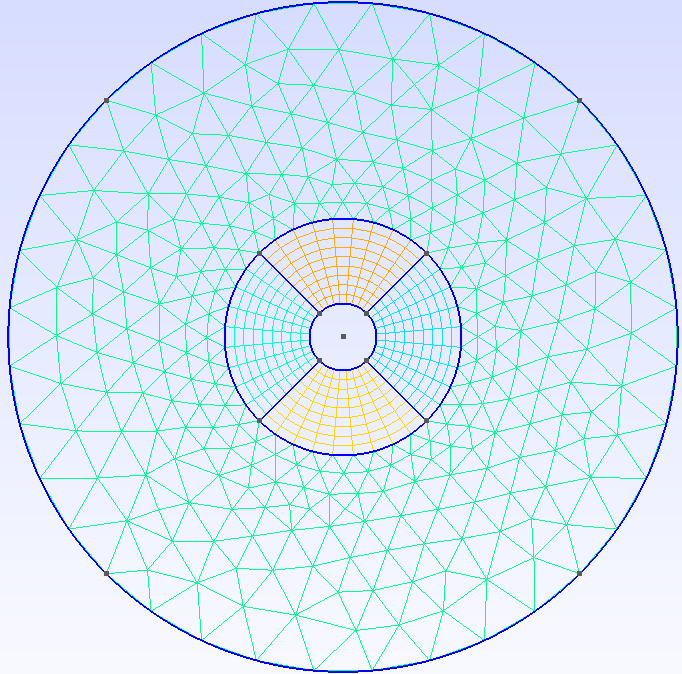
\includegraphics[width=0.4\linewidth]{HW2/Test Mesh Provided.png}
    \caption{Provided Mesh}
\end{figure} \par

The second mesh consists of the same boundary geometries as the first mesh discussed above. However, unlike the first mesh, this mesh has a square in the middle. Furthermore, quadrilateral elements are pushed towards the outer region while triangular elements are pulled inside the square. This mesh is constructed to see the effect of decreasing symmetry planes on the $L_2$ norm. \\\par

\begin{figure}[h]
    \centering
    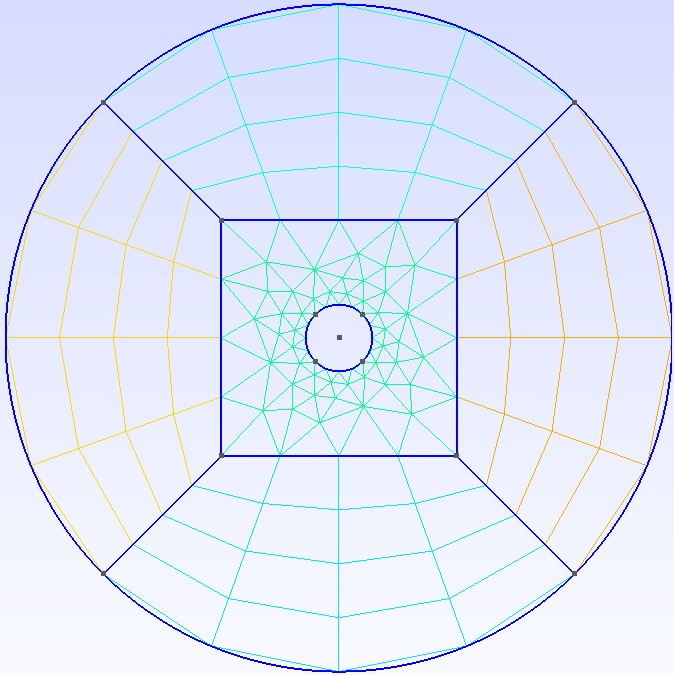
\includegraphics[width=0.4\linewidth]{HW2/Circles with Square Middle.jpg}
    \caption{Circle with Square Middle}
\end{figure}\par

The third mesh is constructed with a quadrilateral shape in the middle. The inner and outer boundary geometries are the same as in the first mesh. The geometry resembles a compass hence it is named after it. There are triangular meshes in the inner and quadrilateral elements outwards. This mesh is constructed to see whether symmetry is distorted between planes and affects the $L_2$ norm.\\\par 

\begin{figure}[h]
    \centering
    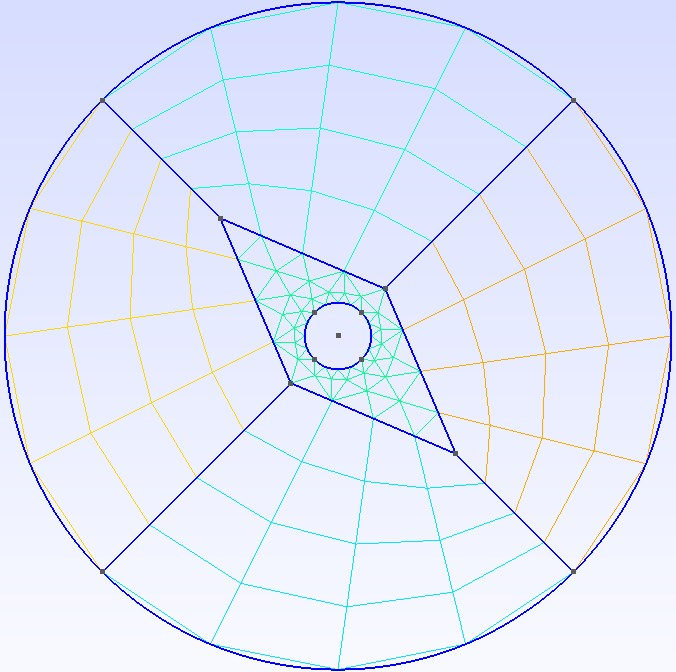
\includegraphics[width=0.4\linewidth]{HW2/Compass .jpg}
    \caption{Compass Like Middle}
\end{figure}\par


The fourth mesh is the distorted version of the previous one. This mesh has properties similar to the previous one. However, it differs in terms of symmetry, as one can observe from the below figure, there are no planes of symmetry.\\\par


\begin{figure}[h]
    \centering
    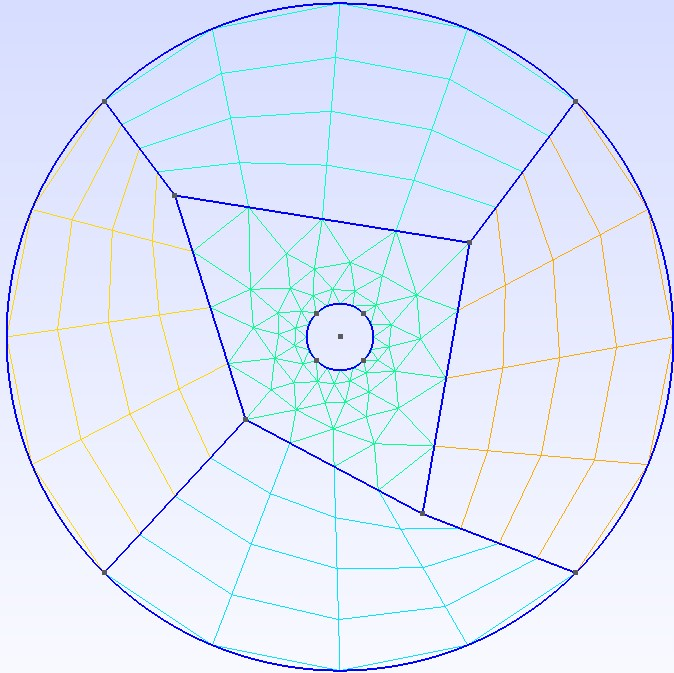
\includegraphics[width=0.4\linewidth]{HW2/Down Compass.jpg}
    \caption{Distorted Compass Like Middle}
    \label{mesh4}
\end{figure}\par

From here on there will be no normal mesh types, only Kershaw mesh types will be presented. These were rather easy to implement since only $\alpha$ values are changing in between meshes. Respectively, values of $\alpha$ will be gradually increased from [0.2, 0.3, 0.5, 0.7]. It is expected to see a structured mesh when $\alpha$ is selected as 0.5, and our first insight is to see close $L_2$ norms in between $\alpha$ values 0.3 and 0.7. We expect to see this trend since basically they are nearly symmetric of each other. \\\par


\begin{figure}[h]
\centering
\begin{minipage}{.5\textwidth}
  \centering
  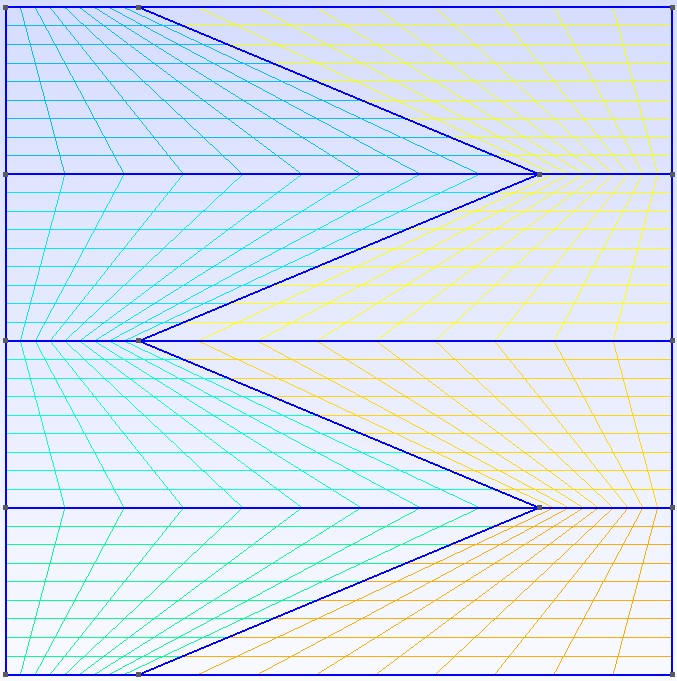
\includegraphics[width=.4\linewidth]{HW2/Kershaw 0.2.jpg}
  \captionof{figure}{$\alpha = 0.2$}
  \label{mesh5}
\end{minipage}%
\begin{minipage}{.5\textwidth}
  \centering
  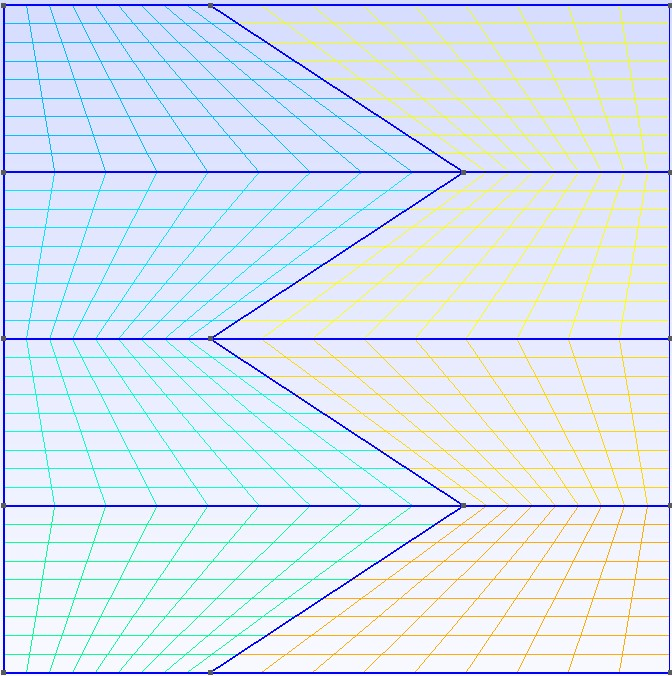
\includegraphics[width=.4\linewidth]{HW2/Kershaw 0.3.jpg}
  \captionof{figure}{$\alpha = 0.3$}
\end{minipage}
\end{figure}
\begin{figure}[h]
\centering
\begin{minipage}{.5\textwidth}
  \centering
  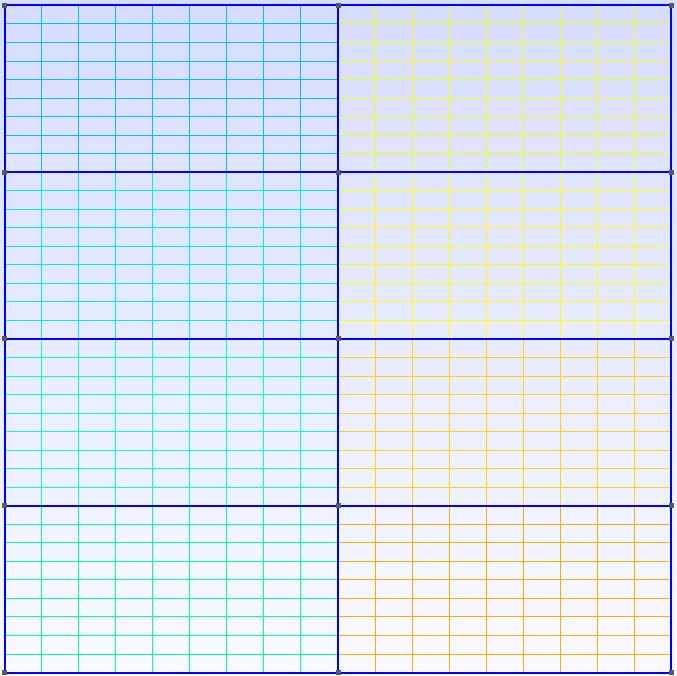
\includegraphics[width=.4\linewidth]{HW2/Kershaw 0.5.jpg}\label{Kershaw Meshes}
  \captionof{figure}{$\alpha = 0.5$}
\end{minipage}%
\begin{minipage}{.5\textwidth}
  \centering
  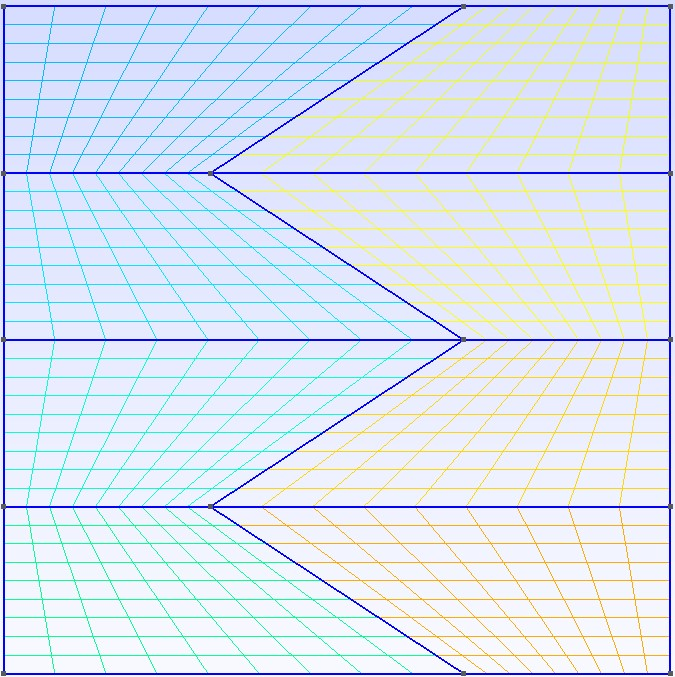
\includegraphics[width=.4\linewidth]{HW2/Kershaw 0.7.jpg}
  \captionof{figure}{$\alpha = 0.7$}
\end{minipage}
\end{figure}


Furthermore, the meshes are summarized in \hyperref[mesh]{\textit{table 3}} for easy following.

\subsection{$L_2$ Error Norms}
In this section, the $L_2$ error norms are tabulated with 2 different initial and boundary condition sets. One "cooling" and one "heating". This paper defines the "heating" case as the given case of $q_{ic} = 0 ,\:q_{inner} = 0,\:q_{outer}=1$ and "cooling" as the opposite, meaning $q_{ic} = 1 ,\:q_{inner} = 1,\:q_{outer}=0$. \\\par
Furthermore, the boundary types are set as Drichlet as, unfortunately, the exact solution for Neumann boundary condition could not be determined with out limited calculus skills and time. \\\par
The tables for cases \hyperref[hot]{\textit{"heating"}} and \hyperref[cold]{\textit{"cooling"}} are presented in the next two pages.
\newpage
\begin{table}[h]
    \renewcommand\baselinestretch{1.1}\selectfont
    \centering
    \mbox{}\clap{
    \begin{tblr}
        []{
        rowsep =1mm,
        colspec = {Q[c,m, 2cm]Q[c,m,4.7cm]Q[c,m,4.7cm]Q[c,m,4.7cm]},
        vlines, hlines,
        row{1} = {gray9}
        }
        Mesh & $L_2$ Error Norm (Minimum) & $L_2$ Error Norm (Orthagonal) & $L_2$ Error Norm (Over-Relaxed)  \\
        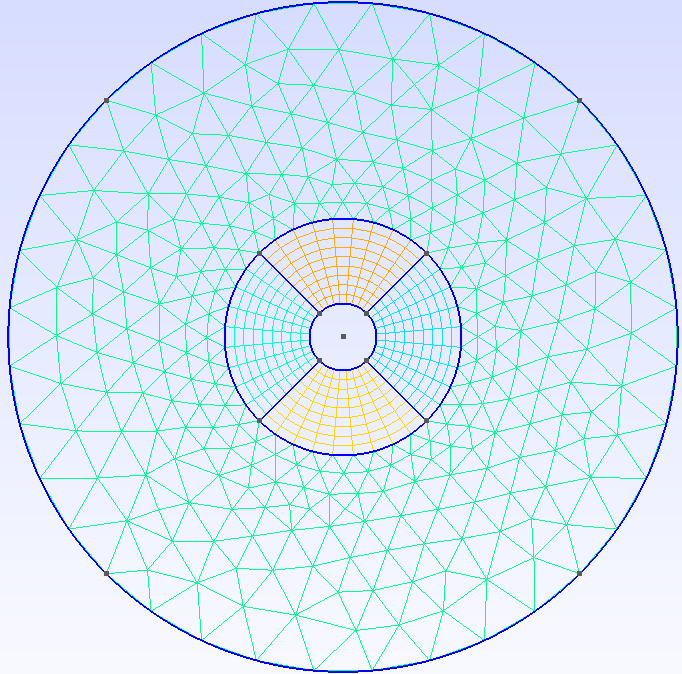
\includegraphics[width=0.4\linewidth, align=c]{HW2/Test Mesh Provided.png} Figure 1 & {[0.000722529]} & {[0.000717858]} & {[0.000713203]}\\
        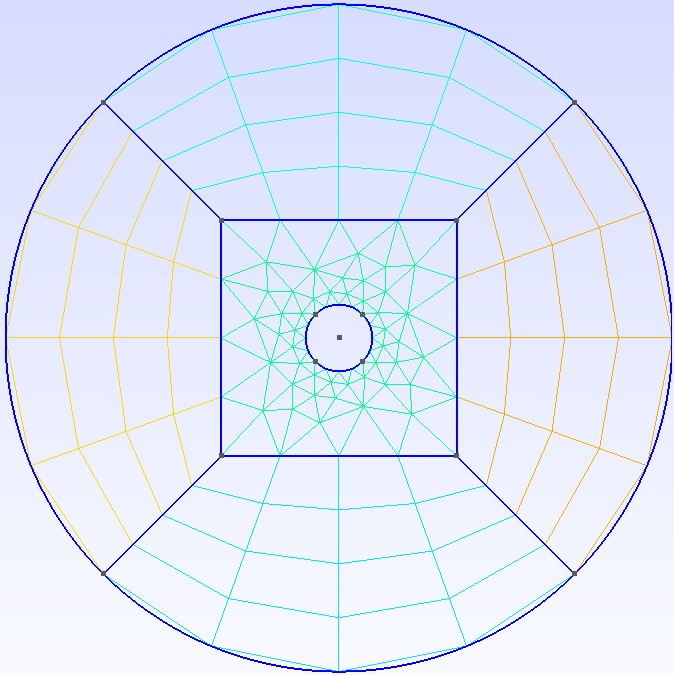
\includegraphics[width=0.4\linewidth, align=c]{HW2/Circles with Square Middle.jpg} Figure 2 & {[0.001150950]} & {[0.001132288]} & {[0.001113778]}\\
        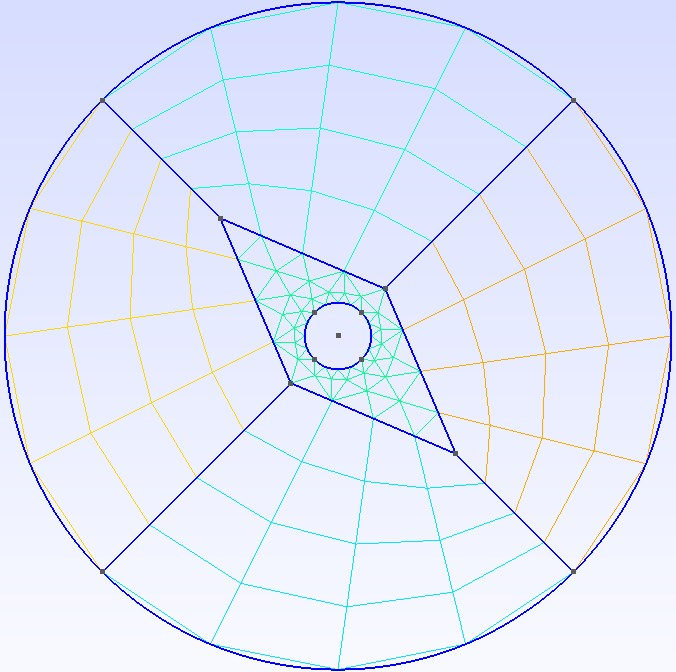
\includegraphics[width=0.4\linewidth, align=c]{HW2/Compass .jpg} Figure 3 & {[0.001603565]} & {[0.001576355]} & {[0.001548625]}\\
        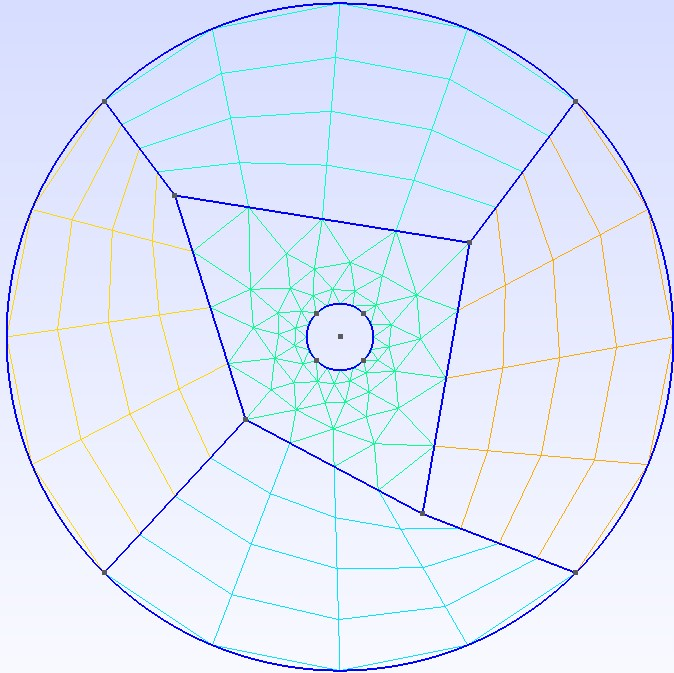
\includegraphics[width=0.4\linewidth, align=c]{HW2/Down Compass.jpg} Figure 4 & {[0.001236185]} & {[0.001186776]} & {[0.001138029]}\\
        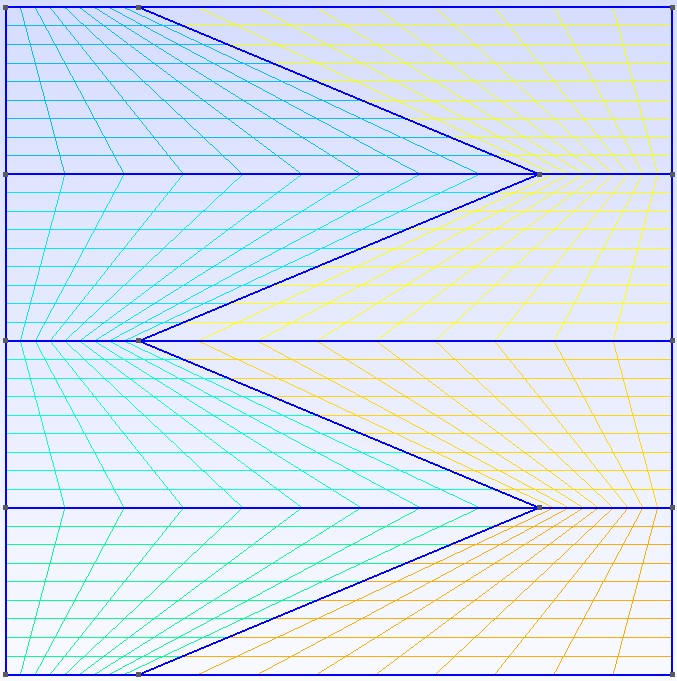
\includegraphics[width=0.4\linewidth, align=c]{HW2/Kershaw 0.2.jpg} Figure 5 & {[4.73146e-11]} & {[4.77808e-11]} & {[4.84148e-11]}\\
        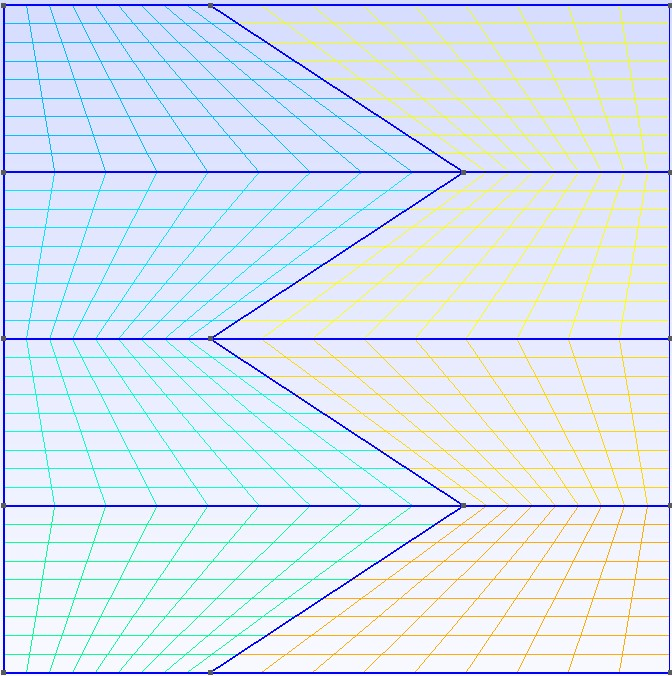
\includegraphics[width=0.4\linewidth, align=c]{HW2/Kershaw 0.3.jpg} Figure 6 & {[6.21990e-12]} & {[6.42256e-12]} & {[6.23417e-12]}\\
        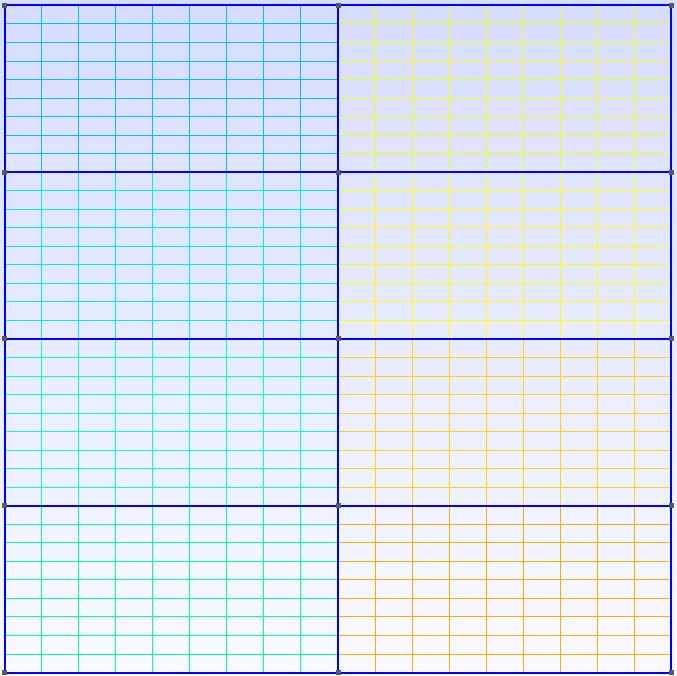
\includegraphics[width=0.4\linewidth, align=c]{HW2/Kershaw 0.5.jpg} Figure 7 & {[3.00667e-12]} & {[3.00605e-12]} & {[3.00612e-12]}\\
        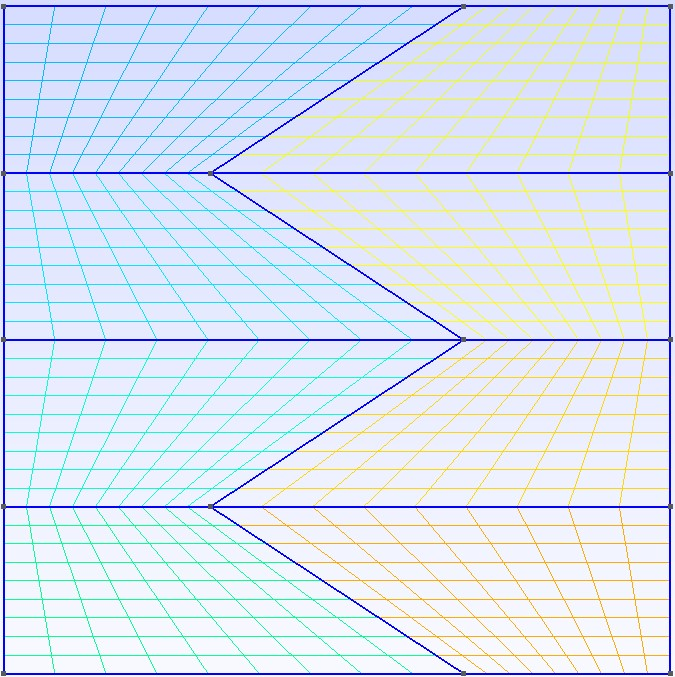
\includegraphics[width=0.4\linewidth, align=c]{HW2/Kershaw 0.7.jpg} Figure 8 & {[6.24074e-12]} & {[6.26951e-12]} & {[6.25994e-12]}\\
    \end{tblr}
    }
    \caption{Results for $q_{ic} = 0 ,\:q_{inner} = 0,\:q_{outer}=1$ Dirichlet}
    \label{hot}
\end{table}
\newpage
\begin{table}[h]
    \renewcommand\baselinestretch{1.1}\selectfont
    \centering
    \mbox{}\clap{
    \begin{tblr}
        []{
        rowsep =1mm,
        colspec = {Q[c,m, 2cm]Q[c,m,4.7cm]Q[c,m,4.7cm]Q[c,m,4.7cm]},
        vlines, hlines,
        row{1} = {gray9}
        }
        Mesh & $L_2$ Error Norm (Minimum) & $L_2$ Error Norm (Orthagonal) & $L_2$ Error Norm (Over-Relaxed)  \\
        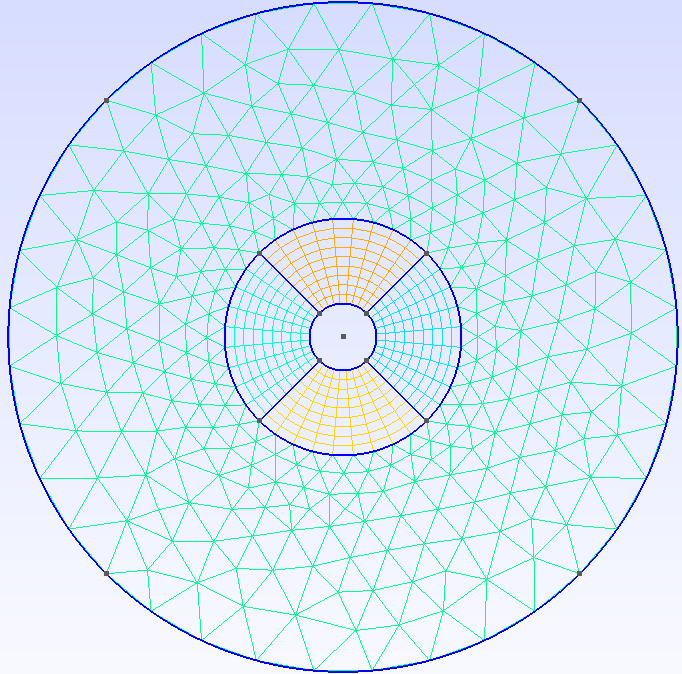
\includegraphics[width=0.4\linewidth, align=c]{HW2/Test Mesh Provided.png} Figure 1 & {[0.000722529]} & {[0.000717858]} & {[0.000713203]}\\
        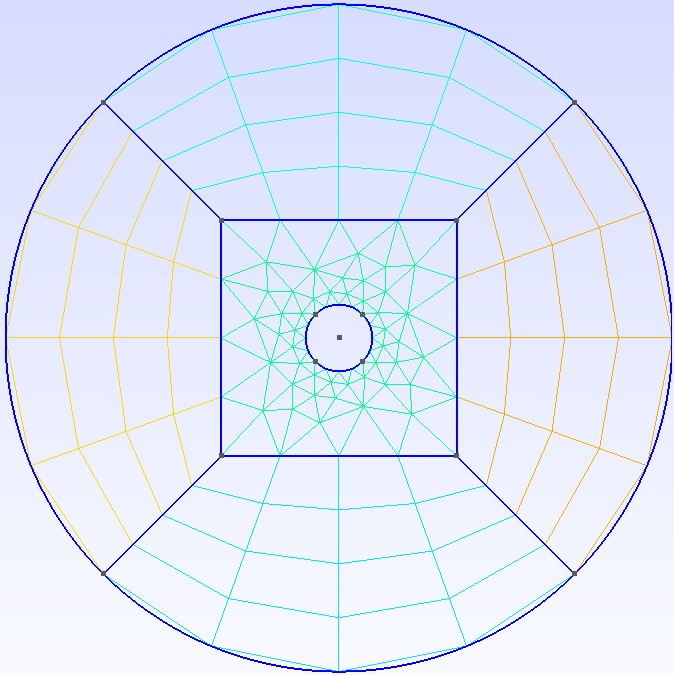
\includegraphics[width=0.4\linewidth, align=c]{HW2/Circles with Square Middle.jpg} Figure 2 & {[0.001150950]} & {[0.001132288]} & {[0.001113778]}\\
        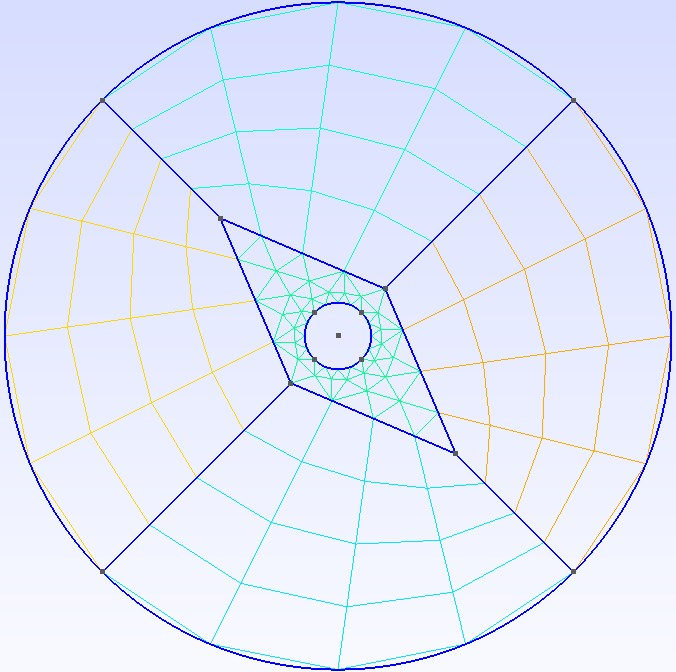
\includegraphics[width=0.4\linewidth, align=c]{HW2/Compass .jpg} Figure 3 & {[0.001603565]} & {[0.001576355]} & {[0.001548625]}\\
        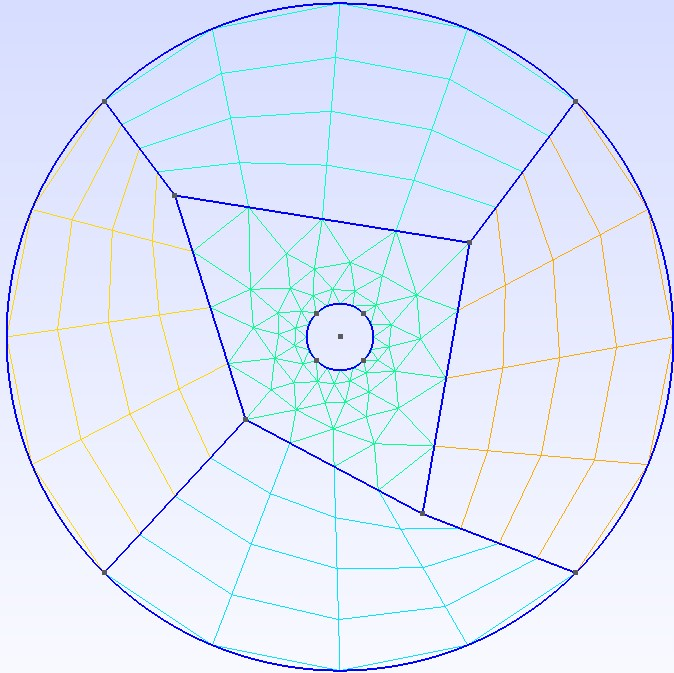
\includegraphics[width=0.4\linewidth, align=c]{HW2/Down Compass.jpg} Figure 4 & {[0.001236185]} & {[0.001186776]} & {[0.001138029]}\\
        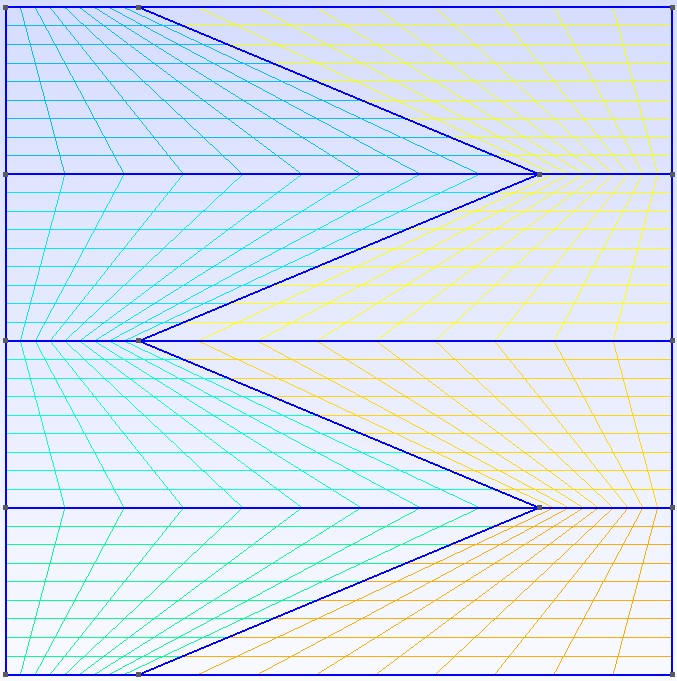
\includegraphics[width=0.4\linewidth, align=c]{HW2/Kershaw 0.2.jpg} Figure 5 & {[4.73146e-11]} & {[8.81601e-12]} & {[8.43790e-12]}\\
        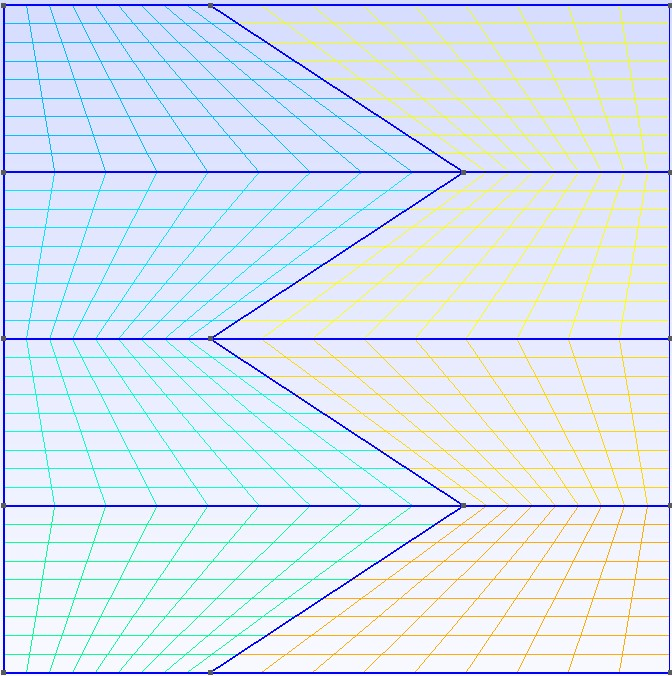
\includegraphics[width=0.4\linewidth, align=c]{HW2/Kershaw 0.3.jpg} Figure 6 & {[1.10656e-12]} & {[1.08697e-12]} & {1.04969e-12}\\
        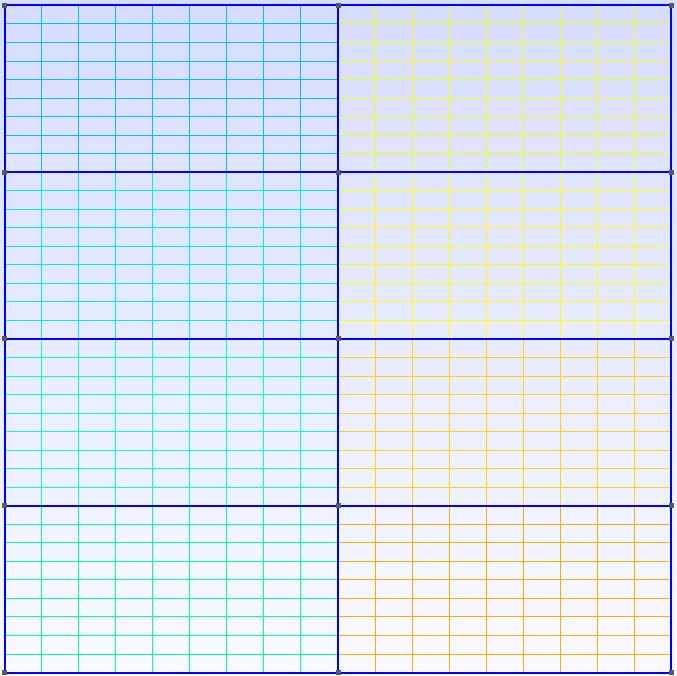
\includegraphics[width=0.4\linewidth, align=c]{HW2/Kershaw 0.5.jpg} Figure 7 & {[4.86977e-13]} & {[4.86467e-13]} & {[4.85080e-13]}\\
        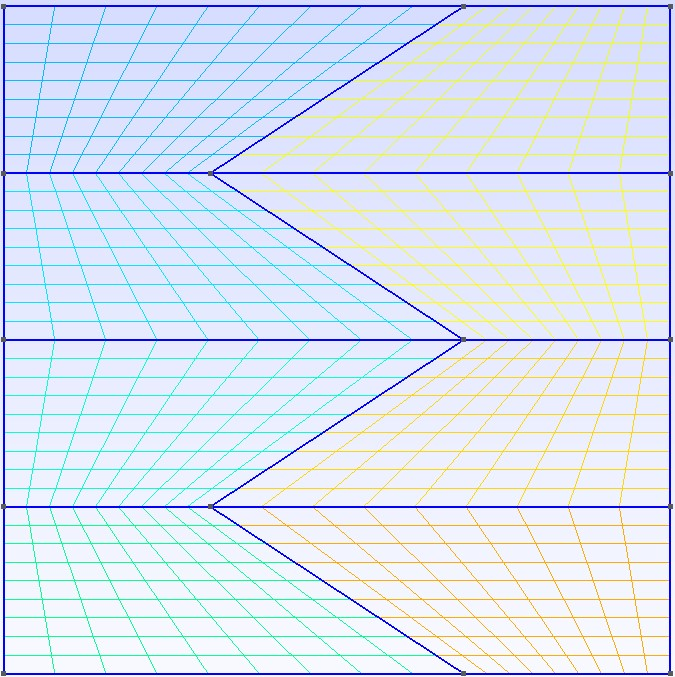
\includegraphics[width=0.4\linewidth, align=c]{HW2/Kershaw 0.7.jpg} Figure 8 & {[1.08052e-12]} & {[1.04127e-12]} & {[1.02194e-12]}\\
    \end{tblr}
    }
    \caption{Results for $q_{ic} = 1 ,\:q_{inner} = 1,\:q_{outer}=0$ Dirichlet}
    \label{cold}
\end{table}\newpage

\subsection{Comments}
The work done follows the initial expectations. The most structured mesh, Kershaw mesh with $\alpha = 0.5$, is expected to have the smallest $L_2$ norm. In addition, one can go to \hyperref[hot]{\textit{Table 1}}  or \hyperref[cold]{\textit{Table 2}} to see the trend of decreasing $L_2$ norm towards the \hyperref[Kershaw Meshes]{\textit{Kershaw mesh with $\alpha = 0.5$}} . \\\par

Continuing with the tables, when a quick gaze is taken on tables, one can see a sharp increase of an order of magnitude when \hyperref[mesh4]{\textit{test mesh 4}}  and \hyperref[mesh5]{\textit{test mesh 5}} are compared. This "jump" happens because the method is switched to Kershaw mesh generation. One can conclude that despite having longer computation time, Kershaw mesh generation has better results. \\\par

Another comparison can be made between normal meshes. As symmetry planes of the test mesh decreases, $L_2$ norm tend to increase. The smallest $L_2$ norm is obtained from the test mesh provided since it has infinitely large symmetry plane number. \\\par

A general comparison can be made in between \hyperref[hot]{\textit{Table 1}} and \hyperref[cold]{\textit{Table 2}}. The first table indicates a heating problem, and the second table is a cooling problem with different boundary conditions. One remark is when "unsteadiness" is concerned, it is found out that the heating case doesn't reach to steady state until the end of the time step chosen. This causes \hyperref[cold]{\textit{Table 2}} to have lesser $L_2$ norm values.\\\par

As a last comment, the comparison correction methods will be discussed. As can be seen from the \hyperref[hot]{\textit{Table 1}}, for the first five test meshes $L_2$ norm decreases as the method shifts from Minimum to Over-Relaxed. For \hyperref[mesh]{\textit{mesh 6 and 8}}, it first increases then decreases. However for the \hyperref[mesh]{\textit{mesh 7}} the lowest $L_2$ norm is reached with the Orthogonal method since the mesh is structured. When it comes to \hyperref[cold]{\textit{Table 2}} the trend is simple, $L_2$ norm decreases as the method shifts from Minimum to Over-Relaxed, and also it decreases as mesh type shifts from normal to Kershaw and unstructured Kershaw to structured Kershaw.

\newpage
\printbibliography
\newpage
\appendix
\section{Mesh Table}
\begin{table}[h]
    \renewcommand\baselinestretch{1.1}\selectfont
    \centering
    \mbox{}\clap{
    \begin{tblr}[]{
        rowsep = 1mm,
        colspec = {Q[c,m, 2cm]Q[c,m,4.7cm]Q[c,m,4.7cm]Q[c,m,4.7cm]},
        vlines, hlines,
        row{1} = {gray9}
        }
         Mesh & Element Count & Node Count & Reason \\
         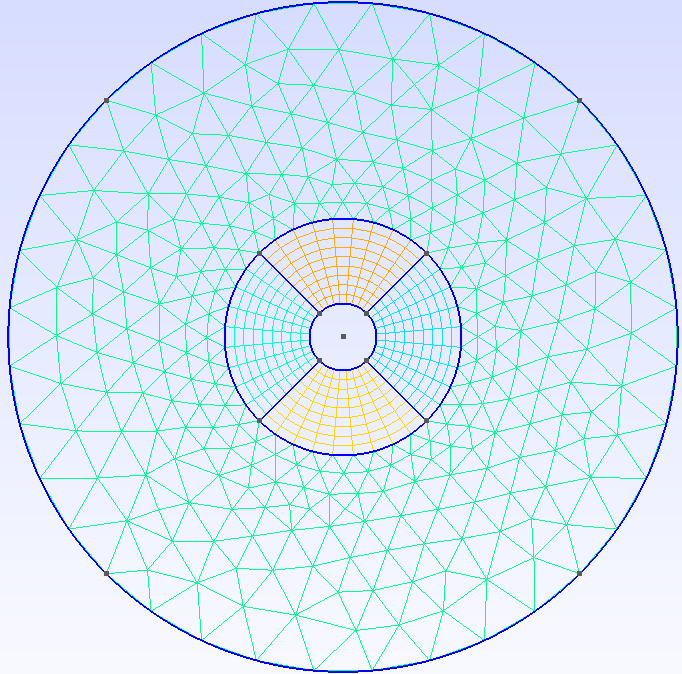
\includegraphics[width=0.4\linewidth, align=c]{HW2/Test Mesh Provided.png} Figure 1 & 1011 & 626 & Default mesh \\
         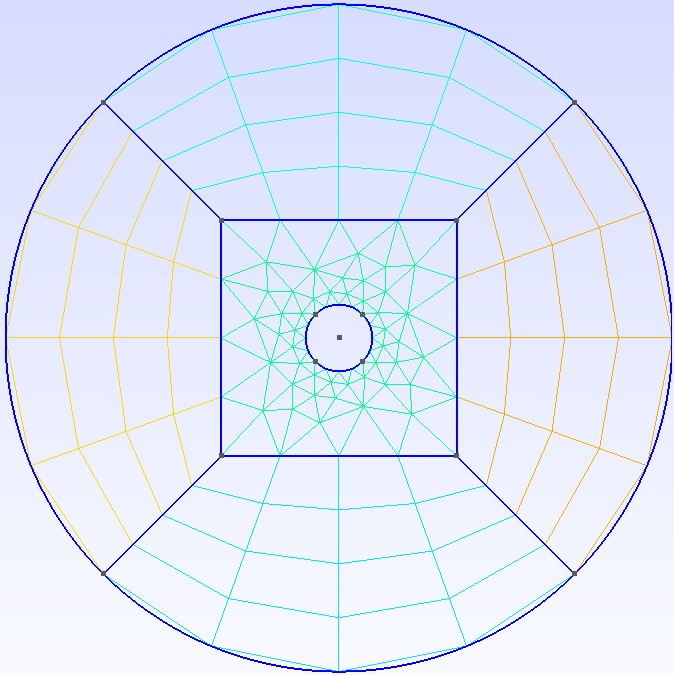
\includegraphics[width=0.4\linewidth, align=c]{HW2/Circles with Square Middle.jpg} Figure 2 & 261 & 141 & Multiple axis of symmetry with both element types. \\
         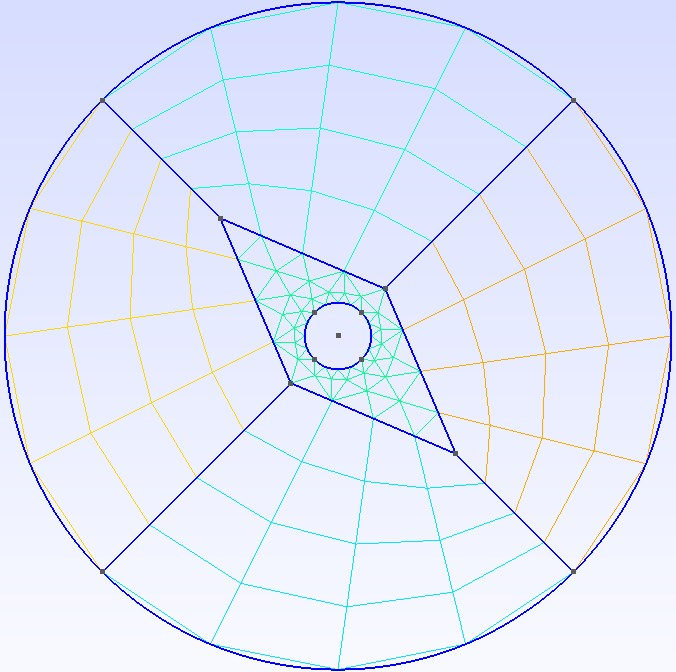
\includegraphics[width=0.4\linewidth, align=c]{HW2/Compass .jpg} Figure 3 & 221 & 121 & Two axis of symmetry with both element types. \\
         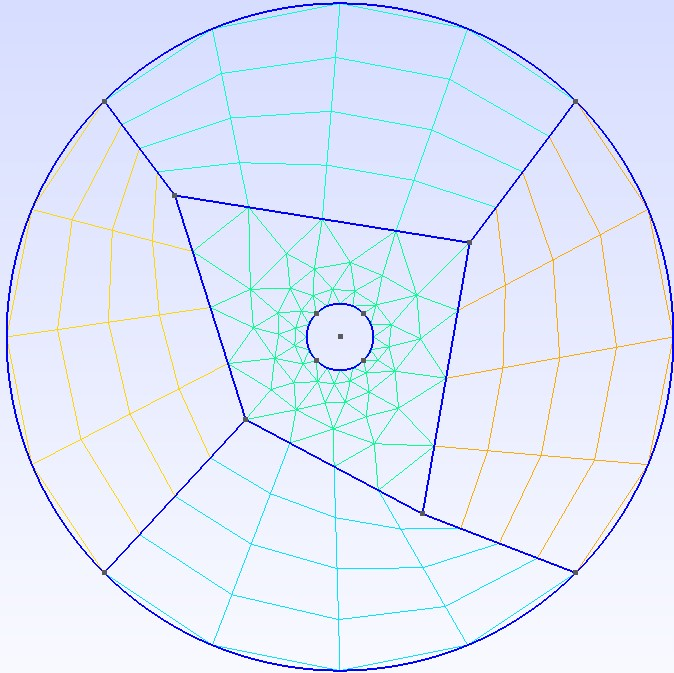
\includegraphics[width=0.4\linewidth, align=c]{HW2/Down Compass.jpg} Figure 4 & 249 & 135 & No axis of symmetry with both element types. \\
         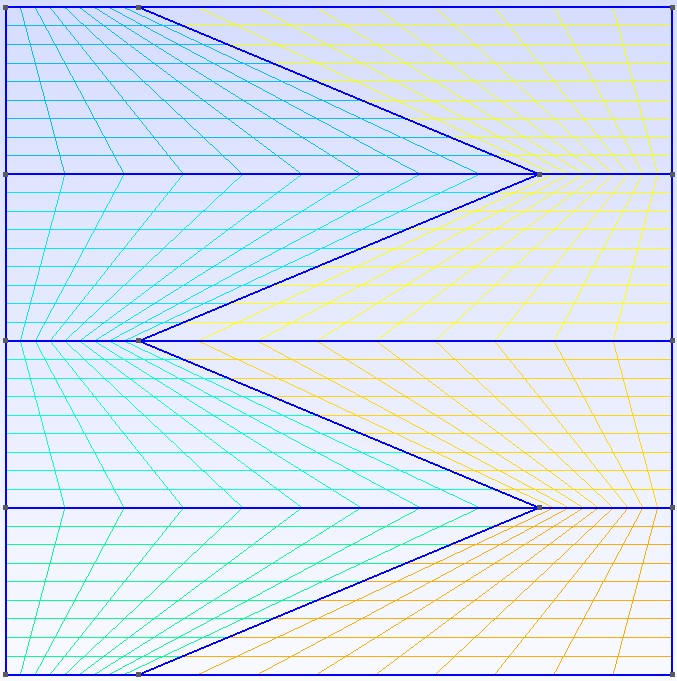
\includegraphics[width=0.4\linewidth, align=c]{HW2/Kershaw 0.2.jpg} Figure 5 & 861 & 703 & Kershaw mesh with $\alpha = 0.2$ \\
         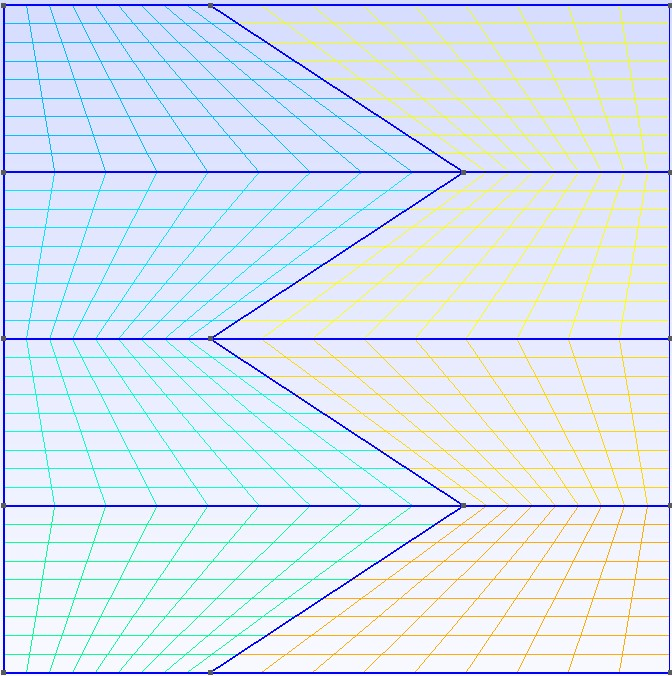
\includegraphics[width=0.4\linewidth, align=c]{HW2/Kershaw 0.3.jpg} Figure 6 & 861 & 703 & Kershaw mesh with $\alpha = 0.3$ \\
         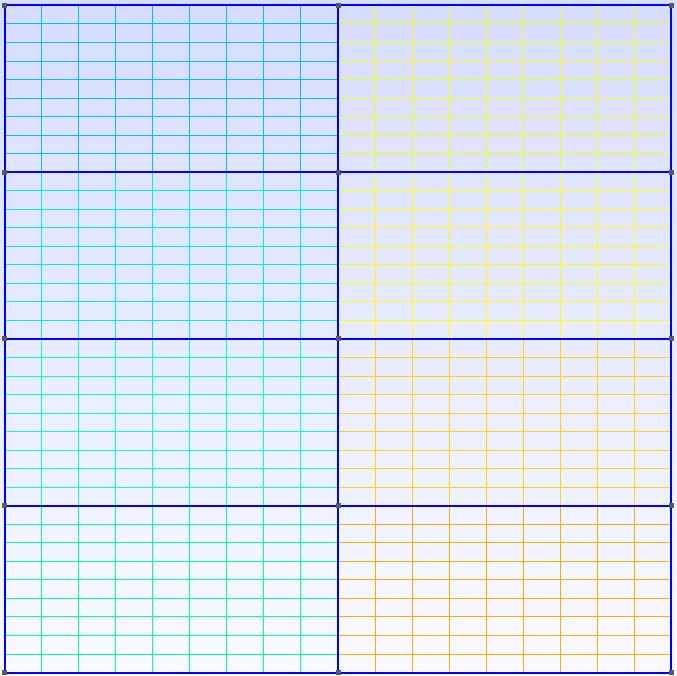
\includegraphics[width=0.4\linewidth, align=c]{HW2/Kershaw 0.5.jpg} Figure 7 & 861 & 703 & Kershaw mesh with $\alpha = 0.5$, structured mesh \\
         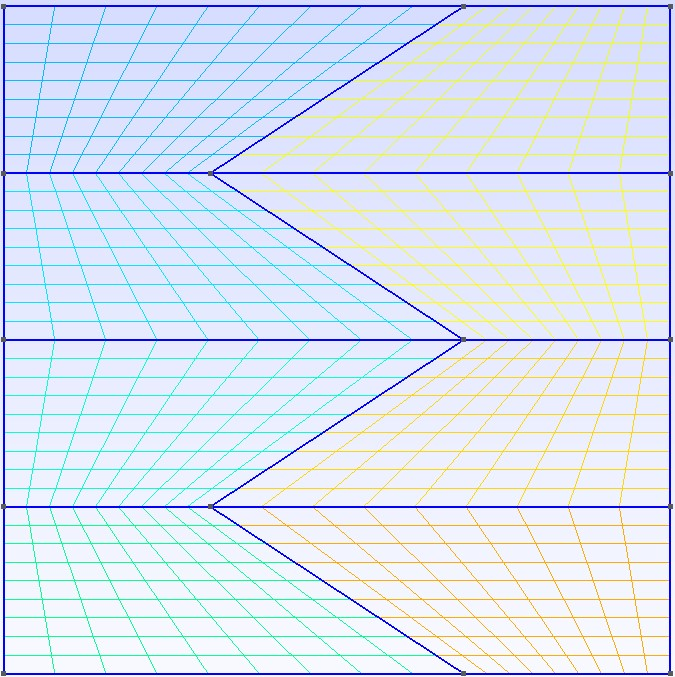
\includegraphics[width=0.4\linewidth, align=c]{HW2/Kershaw 0.7.jpg} Figure 8 & 861 & 703 & Kershaw mesh with $\alpha = 0.7$ \\
    \end{tblr}
    }
    \caption{Statistics of Meshes}
    \label{mesh}
\end{table}
\end{document}